\documentclass[12pt]{article}

\usepackage{mathtools}
\usepackage{bm}
\usepackage{dsfont}
\usepackage{comment}
\usepackage{amssymb}
\usepackage{amsmath}
\usepackage{dsfont}
\usepackage{comment}
\usepackage[nomarkers,figuresonly]{endfloat}
\usepackage{amsfonts}

\usepackage{multirow}
\usepackage{graphicx}
\usepackage{caption}
\usepackage{subcaption}
\usepackage{float}
\usepackage[section]{placeins}
\usepackage[font=normalsize,labelfont=bf]{caption}
\captionsetup[table]{font=footnotesize,labelfont={sf}}

\usepackage{booktabs, siunitx}
\usepackage{array}
\usepackage{accents}
\usepackage{setspace}
\usepackage[round]{natbib}
\usepackage[titletoc]{appendix}


\usepackage{longtable}
\usepackage{totcount}
\usepackage{alphalph}
\usepackage{tabularx}
\usepackage{rotating}

\usepackage{hyperref} 

\usepackage{tikz}
\usetikzlibrary{shapes, arrows.meta, positioning}
\begin{document}
	
\tikzset{%
every neuron/.style={
circle,
draw,
minimum size=1cm
},
neuron missing/.style={
draw=none,
scale=4,
text height=0.333cm,
execute at begin node=\color{black}$\vdots$
},
}

\begin{tikzpicture}[x=1.5cm, y=1.5cm, >=stealth]

\foreach \m [count=\y] in {1,2,3,missing,4}
\node [every neuron/.try, neuron \m/.try] (input-\m) at (0,2.5-\y) {};

\foreach \m [count=\y] in {1,missing,2}
\node [every neuron/.try, neuron \m/.try ] (hidden-\m) at (2,2-\y*1.25) {};

\node[every neuron] (outp) at (4, -.5) {};

\draw[->] (outp) -- ++(1,0) node [above, midway] {$O$};

\foreach \l [count=\i] in {1,2,3,n}
\draw [<-] (input-\i) -- ++(-1,0)
node [above, midway] {$I_\l$};

\foreach \l [count=\i] in {1,n}
\node [above] at (hidden-\i.north) {$H_\l$};

\foreach \i in {1,...,4}
\foreach \j in {1,...,2}
\draw [->] (input-\i) -- (hidden-\j);

\foreach \i in {1,...,2}
\draw [->] (hidden-\i) -- (outp);

\foreach \l [count=\x from 0] in {Input, Hidden, Output}
\node [align=center, above] at (\x*2,2) {\l \\ layer};

\end{tikzpicture}
\newpage 

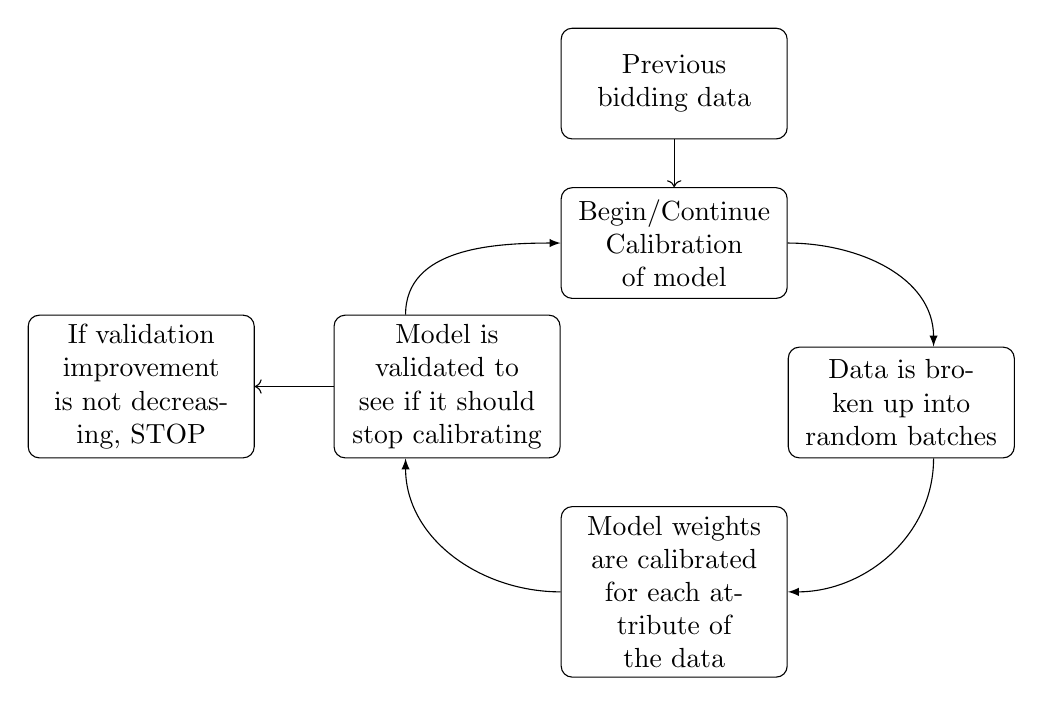
\begin{tikzpicture}[
	node distance=4ex and 0em,
	block/.style={rectangle, draw, fill=white!20, 
		text width=7.5em, text centered, rounded corners, minimum height=4em},
	line/.style={draw, -latex},
	]
	
	\node [block] (0) {Previous bidding data};
	\node [block, below= of 0] (1) {Begin/Continue Calibration of model};
	\node [block, below right= of 1] (2) {Data is broken up into random batches};
	\node [block, below left= of 2] (3) {Model weights are calibrated for each attribute of the data};
	\node [block, above left= of 3] (4) {Model is validated to see if it should stop calibrating};
	\draw [->] (0) -- (1) ;
	\node [block, left = 1cm of 4] (break) {If validation improvement is not decreasing, STOP};
	\draw [->] (4) -- (break) ;  
	\path [line] (1.east) to[out=0, in=90] (2.60);
	\path [line] (2.-60) to[out=-90, in=0] (3.east);
	\path [line] (3.west) to[out=180, in=-90] (4.-120);
	\path [line] (4.120) to[out=90, in=180] (1.west);
\end{tikzpicture}
	\newpage 
	
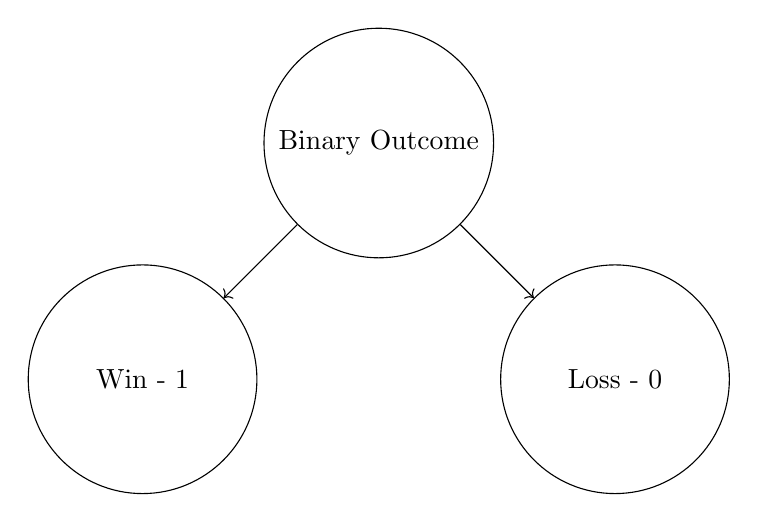
\begin{tikzpicture}[
	node distance=4ex and 0em,
	MyNode/.style={circle, draw, fill=white!20, 
		text width=7.5em, text centered,  minimum height=4em}
	]
	
\node [MyNode] (main) at (0,0) {Binary Outcome}; 
\node [MyNode] (win) at (-3,-3) {Win - 1} ; 
\node [MyNode] (loss) at (3,-3) {Loss - 0} ; 
\draw [->] (main) -- (win);
\draw [->] (main) -- (loss);


\end{tikzpicture}	
\end{document}